\documentclass{llncs}
\usepackage{amssymb}
\usepackage{graphicx}
\usepackage[ruled,linesnumbered,boxed]{algorithm2e}
\usepackage{graphicx}
\usepackage{amsmath}
%\usepackage{mathtools}
%\usepackage{color}
\usepackage{tabularx}
\usepackage[colorlinks, linkcolor=blue, anchorcolor=blue, citecolor=green]{hyperref}
%\usepackage{booktabs}
\usepackage[table]{xcolor}
%\uespackage{colortbl}
\usepackage[tight,footnotesize]{subfigure}
\usepackage{fancyhdr}
\usepackage{lastpage}
\usepackage{layout}
%\usepackage{ctex}

%\footskip = 10pt
\pagestyle{fancy}
\chead{Group Project}
\lhead{CS214-Algorithm@SJTU}
\rhead{Instructor: Xiaofeng Gao}
\rfoot{}
\cfoot{Page \thepage \ of \pageref{LastPage}}
\addtolength{\headheight}{0.5\baselineskip}
\addtolength{\headwidth}{0\marginparsep}
\addtolength{\headwidth}{0\marginparwidth}



\title{Package Delivery on ``Double 11'' Day}
\subtitle{Project for Algorithm and Complexity \vspace{-3mm}}

\author{
Kylin Chen (517030910155, k1017856853@icloud.com) \\
Fangyu Ding (517030910235, arthur\_99@sjtu.edu.cn) \\
Hongzhou Liu (517030910214, deanlhz@sjtu.edu.cn)
  }

\institute{Department of Computer Science, \\ Shanghai Jiao Tong University, Shanghai, China}

\begin{document}
\bibliographystyle{splncs}

%\linespread{0.85}

%==============================================================================
\maketitle
\begin{abstract}\vspace{-5mm}
Package delivery is such a significant problem nowadays. The convenience and speediness of online shopping highly rely on an efficient and well-organized delivery network.
Meanwhile, the delivery companies always want to reduce the cost of transportation while winning high rates from customers. The problem can be modelled as min-cost commodity flows over time.
The characteristics of such kind of problem are networks with capacities and transit times. We also have other properties like the priority of orders of commodities, the ordering time and transportation restrictions 
with respect to special kinds of commodities. However, such kind of problems is really hard to solve. Though static $s$-$t$ flow problem can be solved in polynomial time, the problem we encountered is almost NP-Hard with enormous input size.
Thus, we came up with some approximations to get good feasible solutions, applied these algorithms in different scenes and compared their performance.

\textbf{Keywords:} Package Delivery, Network Flow, Routing, Flow over time.
\end{abstract}

\setcounter{section}{-1}
\section{Symbol Table}
Define all the symbols that will be used later.
\begin{table}
\caption{Symbol Table}\label{sym1}
\centering
\begin{tabular}{|l|l|}
\hline
Symbol &  Attribute \\
\hline
$city$ & $index$, $kind(large/small/hub)$, $capacity$\\
\hline
$tool$ & $departure\_city$, $arrival\_city$, $time$, $average\_delay$, $departure\_time$, $unit\_cost$, $type$ \\
\hline
$commodity$ & $index$, $unit\_weight$, $type$ \\
\hline
$order$ & $seller\_city$, $purchaser\_city$, $order\_time$, $commodity\_index$, $amount$, $emergency$ \\
\hline
\end{tabular}
\end{table}
\newpage
\section{Problem 1}
\subsection{Problem Analysis}
In this part SF Express has its substations on all 656 cities covered in the orders. We came up with a network model. Regard $city$ as vertex and $tool$ as edge, 
we can construct a network and simulate the transportation of orders on it. Our cost function is defined as $$C(p)=transport\_time^{rate}  \times transport\_cost$$
Here $p$ is the path that a particular order takes. And we evaluate the path using our cost function by the time the order takes from the time it was made to the time the 
package was sent to the consumer. We add an exponential $rate$ to represent the weight of time in the cost function. \\
The problem is an $NPO$ problem, we give the formal definition as follows:
\begin{itemize}
  \item $I$: The network model $G=(V,E)$ and the set of $order$
  \item $sol$: A set of paths $P$ representing the delivery scheme
  \item $m$: $m(G,order)=\sum_{p \in P}C(p)$
  \item $goal$: $min$
\end{itemize}
We consider that the problem is not a $LP$ or $ILP$ problem. Because the $transport\_time$ here is not linear. For example, there exist some orders that cannot be sent in the same day it was ordered. 
They will be delayed for several days thus the $transport\_time$ of a certain order will be a piecewise function.
So we defined a non-linear object function, and constructed such network model.
\subsection{Algorithm Design}
\begin{algorithm}
  \KwIn{$G$, $source\_city$, $target\_city$, $order\_time$, $arrival\_time$
        , $visited[]$, $path$, $min$, $optimal\_path$, $depth\_limit$}
  \BlankLine
  \caption{$dfs$}
  \label{Alg-dfs-with-depth-limit}
  
  \If{$source\_city == target\_city$ and $path$'s value $< min$ }{
    $min=$ $path$'s value\;
    $optimal\_path = path$\;
    $return$\; 
  }
  \If{$depth\_limit ==0$}{
    $return$\;
  }
  \BlankLine 
  
  $visited[source\_city] = true$\;
  \For{each $(city, out\_way)$ adjacent to $source\_city$}{
    \If{$visited[city]==true$ 
        and $out\_way.departure\_time \ge arrival\_time$}{
          $visited[city] = true$\;
          $path.push\_back(out\_way)$\;
          \BlankLine
          // branch-cutting-off\;
          \If{$path$'s value $< min$}{
            $dfs(G, city, target\_city, order\_time, out\_way.arrival\_time$\\
            $, visited, path, min, optimal\_path, depth\_limit - 1)$\;
          }
          \BlankLine
          $path.pop\_back()$\;
          $visited[city] = false$\;
        }
  }

\end{algorithm}
\subsection{Theoretical Analysis}
\subsubsection{Complexity Analysis}
We implemented a depth-limited DFS algorithm which technically called \textbf{iterative deepening depth-first search(IDDFS)} to search for optimal solutions. 
The time complexity is $O(b^d)$, where $b$ is the branching factor and $d$ is the depth limit.
With a depth limit, the nodes at depth $d$ are expanded once, the nodes at depth $d-1$ are expanded twice. So the total number of expansions in an IDDFS is
$$b^d + 2b^{d-1} + 3b^{d-2} + ... + (d-1)b^2 + db + (d+1) = \Sigma_{i=0}^{d} (d + 1 - i)b^i$$
where $b^d$ is the number of expansions at depth $d$, $2b^{d-1}$ is the number of expansions at depth $d-1$, and so on. Factoring out $b^d$ gives
$$b^d(1 + 2b^{-1} + 3 b^{-2} + ... + (d + 1)^{-d})$$
Now let $x = \frac{1}{b}$, then we have 
$$b^d(1 + 2x + 3x^2 + ... )$$ which converge to 
$$b^d(1 - x)^{-2}$$ for $abs(x) < 1$
Since $(1-x)^{-2}$ is a constant independent of $d$(the depth), if $b > 1$ (i.e., if the branching factor is greater than 1)\\
The time complexity is $O(b^d)$.
Besides, as we also use the strategy of \textbf{branch-cutting-off}, when the total value of the current path IDDFS has found is larger than the current optimal, IDDFS would not carry on searching more cities at this branch.\\
Therefore, the branching factor $b$ would be divided by $2$ because every time we want to carry on searching at one city, half of the out ways would be strictly \textbf{impossible to be optimal} in expectation. As a result, the factor $b$ would be divided by $2$ to be $O((\frac{b}{2})^d)$, which will significantly reduce  the time complexity. 
\subsubsection{Efficiency Analysis}
The problem is an NP problem. We can find such a certifier that given a delivery scheme we can verify the correctness order-by-order. The procedure will take polynomial time and thus the problem is NP.
\subsection{Performance Evaluation}
Problem 1 is a foundation of our project, thus we take a detailed evaluation in this part. \par
First, we will take a look at the time of transfer for the optimal path of each order. Notice that $depth=\#transfer\_time+1$

\begin{figure}[htbp]
  \centering\textbf{}
  \subfigure[max depth = 3]{
  \label{Graph1-1}
  \begin{minipage}[t]{0.3\linewidth}
  \centering
  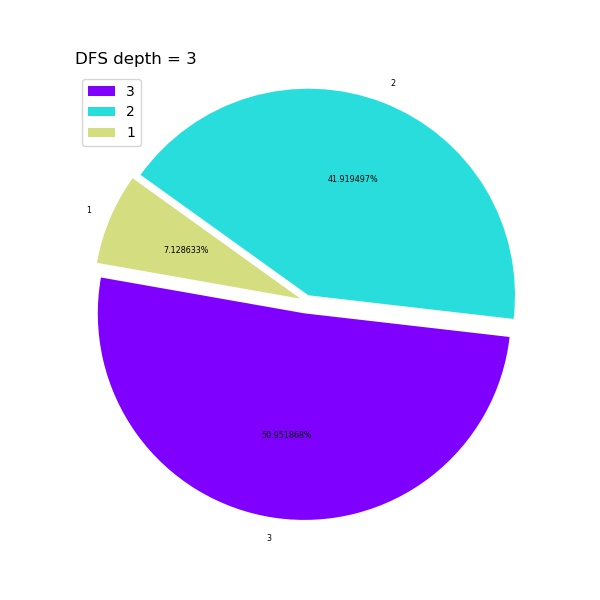
\includegraphics[width=5.5cm]{graph/Demo_official_dfs3.jpg}
  \end{minipage}
  }
  \subfigure[max depth = 4]{
  \begin{minipage}[t]{0.3\linewidth}
  \centering
  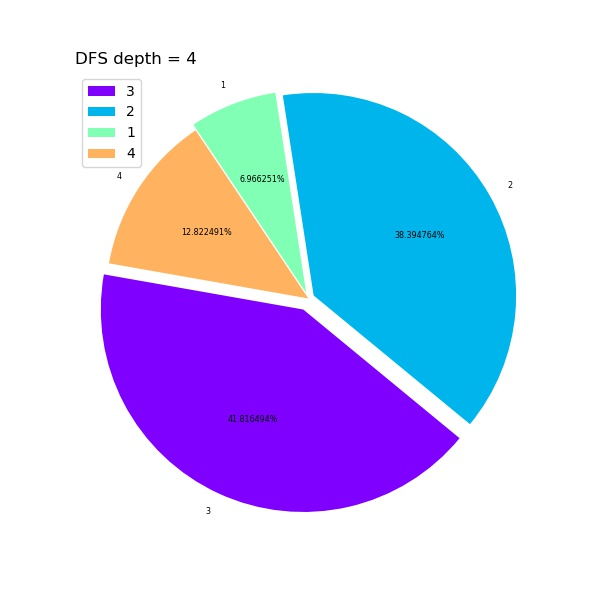
\includegraphics[width=5.5cm]{graph/Demo_official_dfs4.jpg}
  \end{minipage}
  }
  \subfigure[max depth = 6]{
  \begin{minipage}[t]{0.3\linewidth}
  \centering
  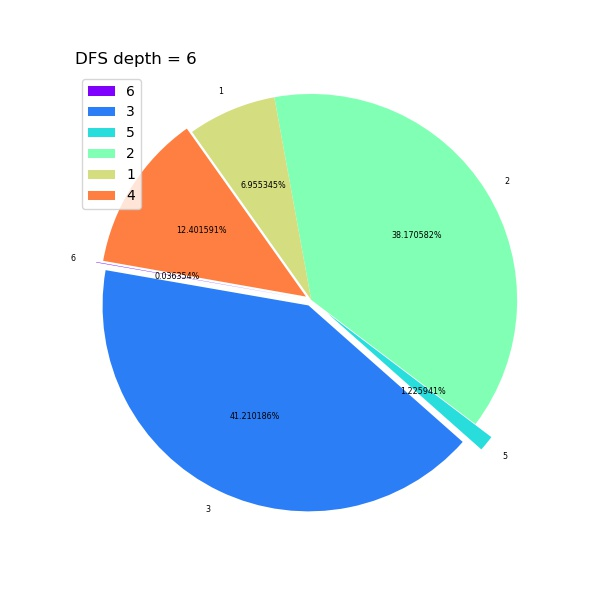
\includegraphics[width=5.5cm]{graph/Demo_official_dfs6.jpg}
  \end{minipage}
  \label{Graph1-3}
  }
  \centering
  \caption{Influence of DFS depth}
\end{figure}

In our algorithm, we set a limitation of search depth. Once a certain order can find its optimal path under this limitation, we are sure it's an optimal solution. If not, we will let those 
orders who will not find it's optimal under the limitation, we will make it wait in some city and find a suboptimal solution.
As we can see in Figure.~\ref{Graph1-1}, with the increasing of limitation of depth, some part our pie chart decreased, which means some suboptimal solutions become more optimal ones due to the increasing 
of the searching limitation. But increasing the limitation will bring us heavily computation cost and the worst circumstance will have limitation of 656, which is unaffordable to find all optimal solutions.
However, we found that the proportion of orders which will take longer path to find their optimal is relatively small, thus we can take smaller depth limitation to make it an approximate algorithm. In Problem 1-3, we will regard the solution with 6 as global optimal solution because we can find the orders with 6 midway-transfer only covers $0.036354\%$ in Figure.~\ref{Graph1-3}, which means that only a very small part of orders need more than 6 times mid-way transfer. \par


Then, we will discuss the choice of parameter $rate$ in our object function $C(p)$. We ran some testing programs and drew a graph to show the effect of our cost function on the decision of choosing paths in our algorithm.
As we can see as long as the increasing of $rate$ the weight of time cost decreased sharply. It means that it will be hard to evaluate the cost if we choose a relatively large $rate$ for it will hide the contribution of time cost.
So we choose $rate=\dfrac{1}{2}$ in our project to make a fair cost function to evaluate the performance.

\begin{figure}[htbp]
  \centering
  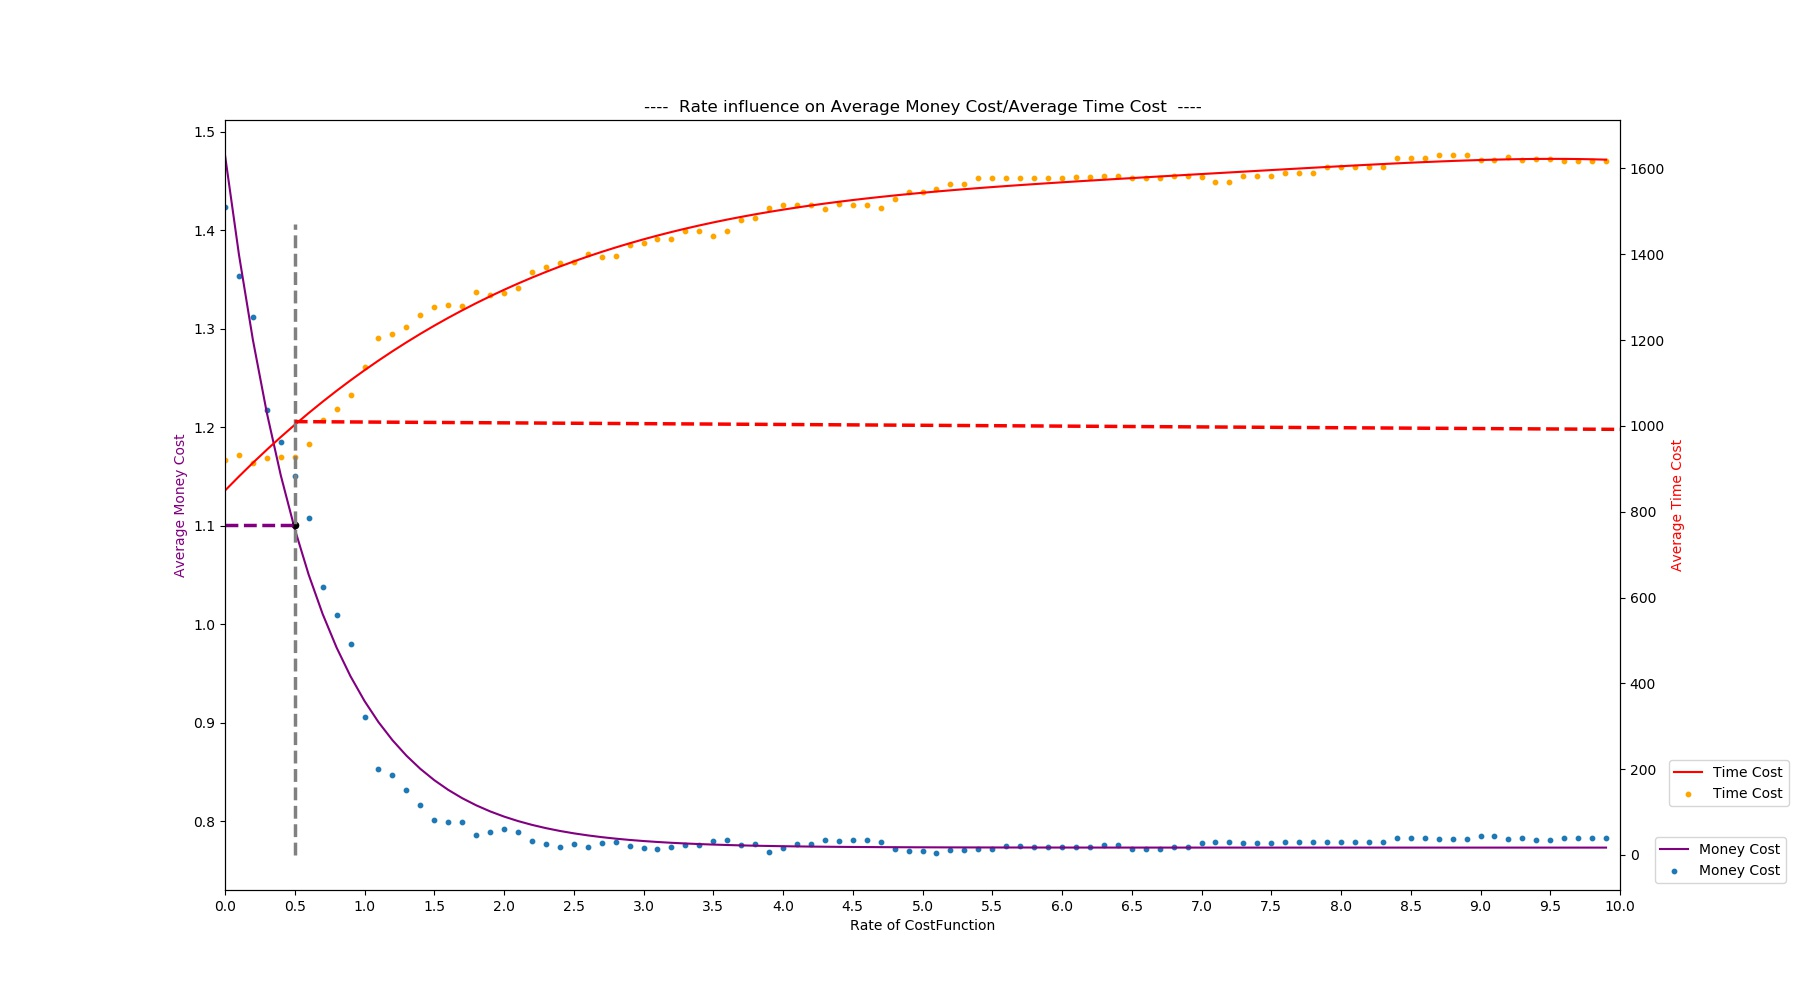
\includegraphics[height = 9cm]{graph/Rate.jpg}
  \caption{Rate}
  \label{fig:rt}
\end{figure}



Finally, we analyze the approximation ratio. As we make the hypothesis that IDDFS with depth=6 can make a global optimal decision for every order, we can use random algorithm to simplify the calculation because IDDFS with 6 will takes much time in dense-edge graph. However, we notice that when we choose the IDDFS depth as 4, our algorithm approximate ratio is strictly under 2. And in this case(with IDDFS depth=4), we can have a best balance between program running time and lower optimal ratio, we can prove it as follows:\par

Even though we get the optimal solution by decreasing cost function C(p), it doesn't have any direct relation with time cost or money cost. So we try to build a random distribution with time cost and money cost respectively rather than with C(p). In the Figure.~\ref{Graph3-0}, we get a distribution of ratio IDDFS4(depth=4) over IDDFS6(depth=6), and we can find the ratio=1 have a very high value which exceed half of all orders, since half of orders in IDDFS4 have reach the optimal solution. But in the approximation analysis, we just want to know what's range the largest proportion covers rather than most single point distribution, so we drop this point and use normalization Gauss Distribution to fix these points like Figure.~\ref{Graph3-1} and Figure.~\ref{Graph3-2}.

\begin{figure}[htbp]
\centering
\begin{minipage}[t]{0.48\textwidth}
\centering
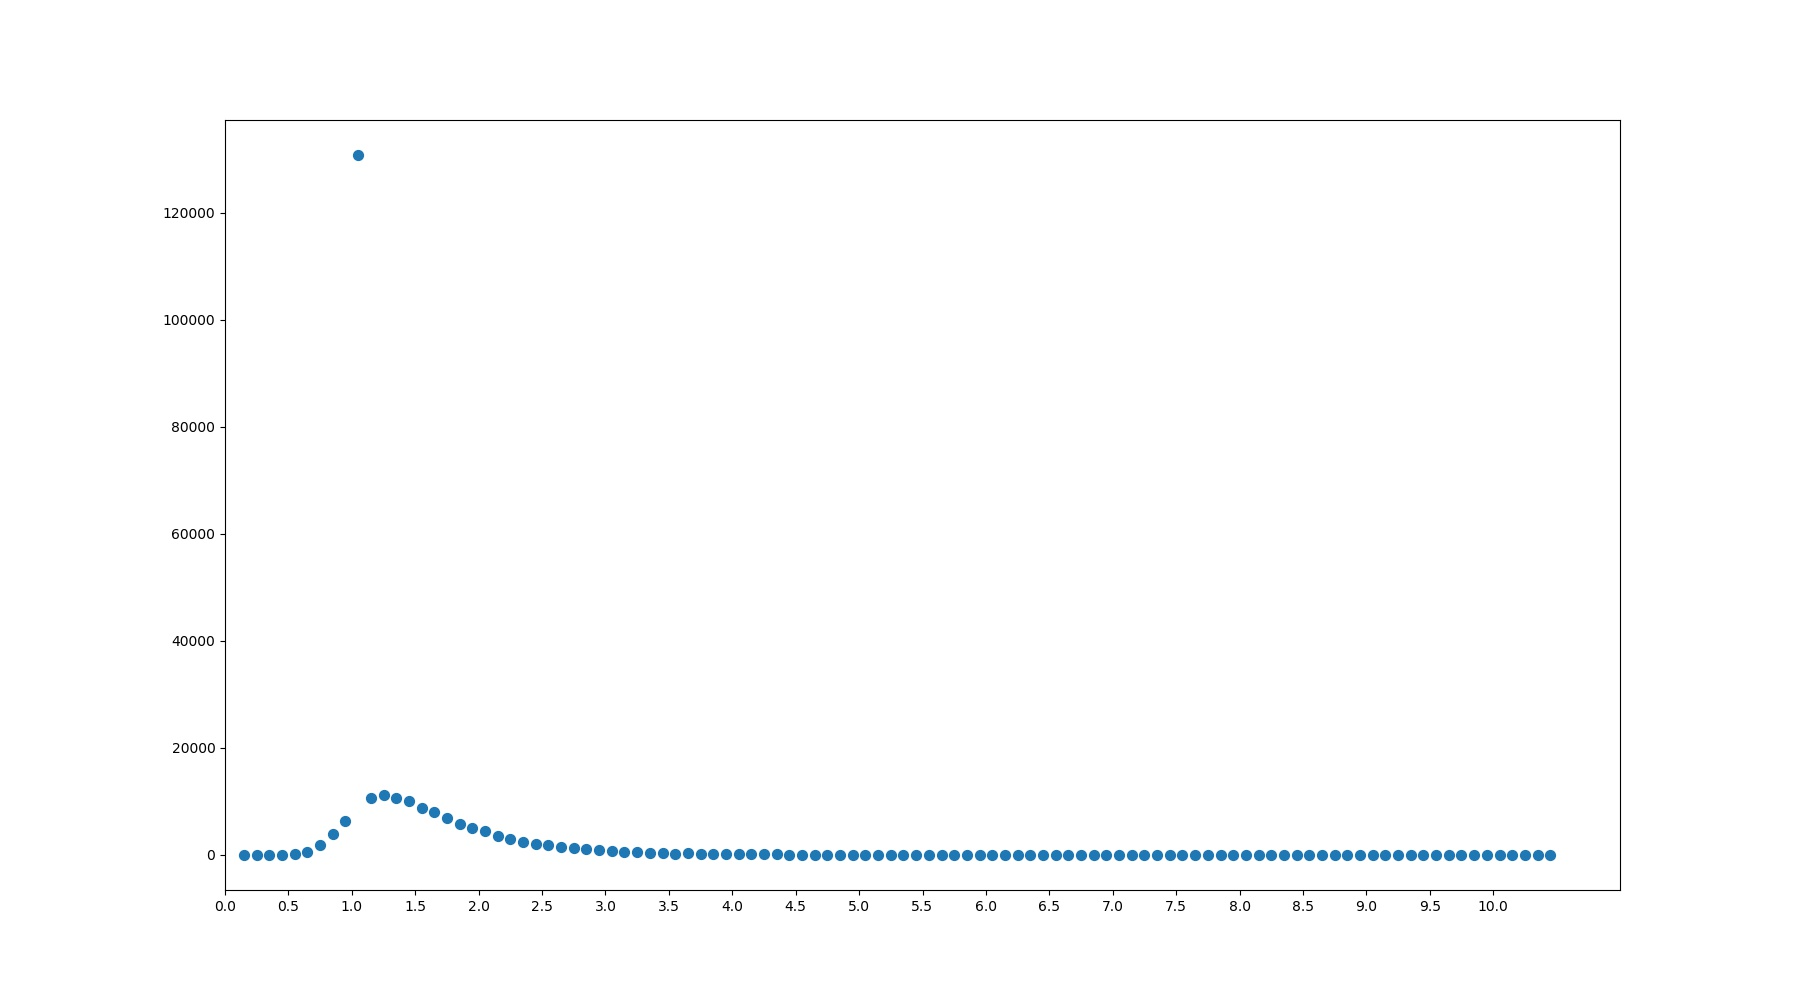
\includegraphics[width = 9cm]{graph/dfs2dfs3_origin.jpg}
\caption{Actual Ratio distribution}
\label{Graph3-0}
\end{minipage}
\begin{minipage}[t]{0.48\textwidth}
\centering
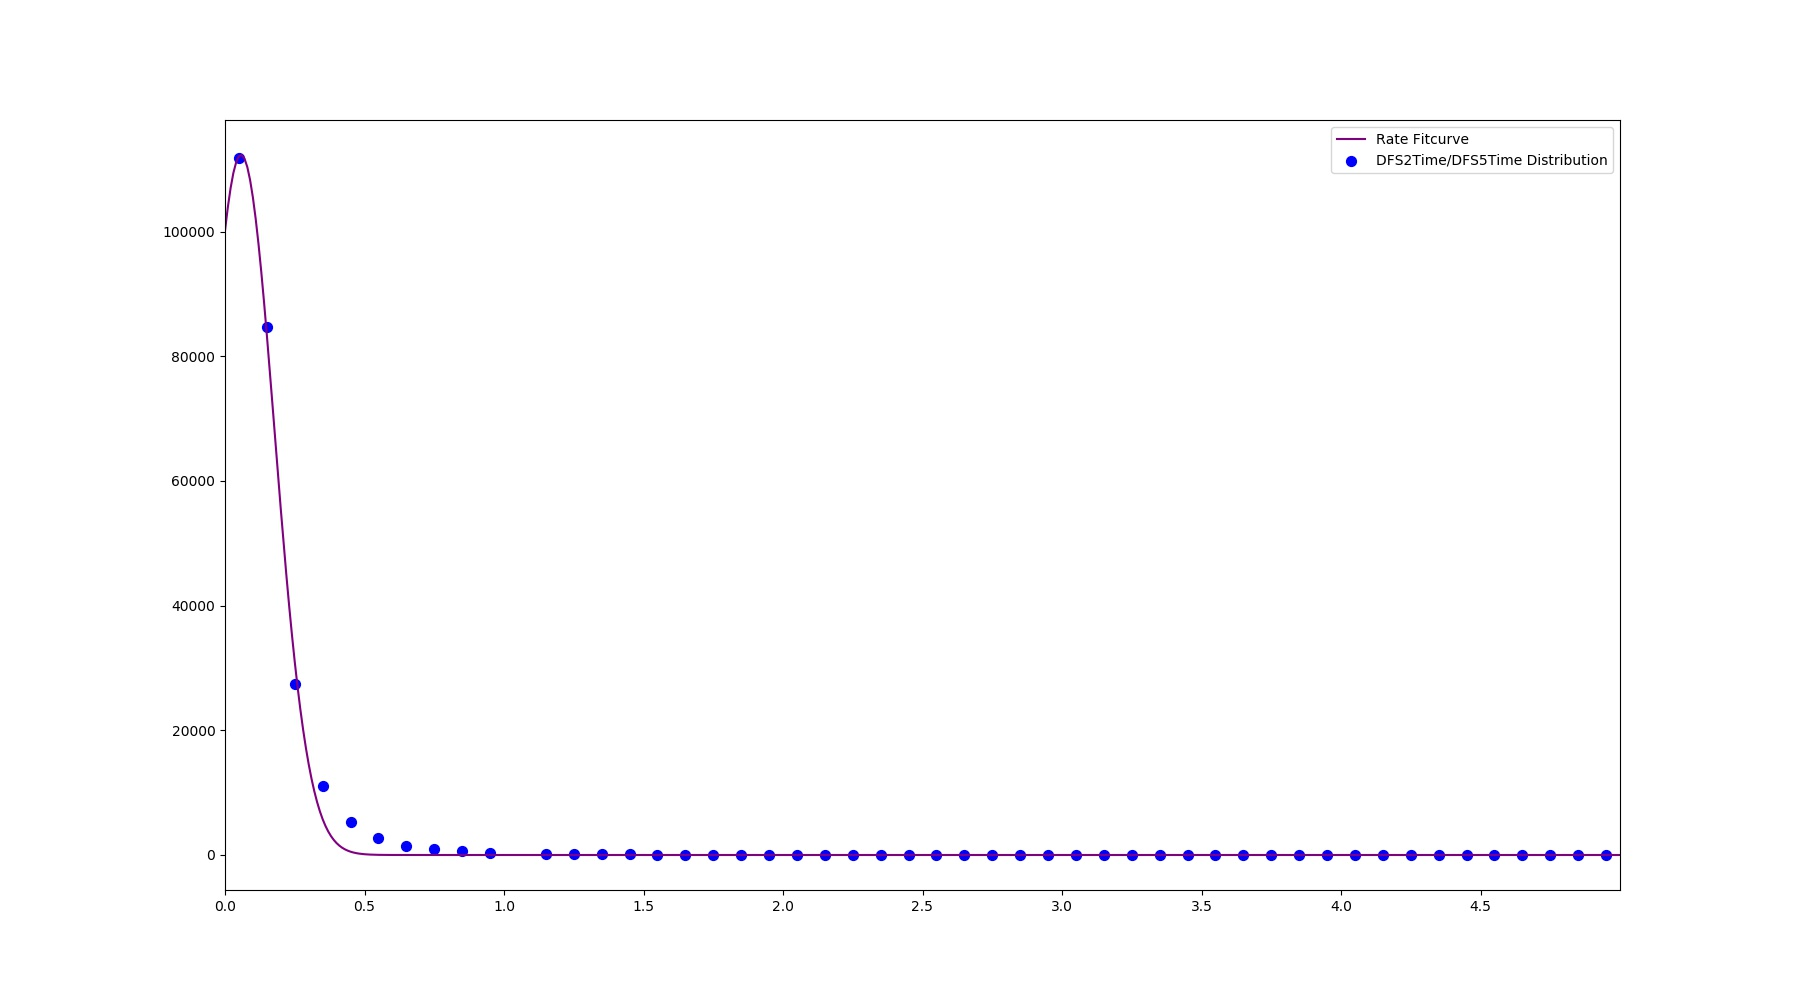
\includegraphics[width = 9cm]{graph/costperday,.jpg}
\caption{Cost/(Day*Weight) Distribution}
\label{Graph3-0-0}
\end{minipage}
\end{figure}

As we can see from Figure.~\ref{Graph3-1} and Figure.~\ref{Graph3-2}, we use normalization Gauss Distribution to fix our ratio DFS4 over DFS6, with Cost and Time respectively. According to Three-Sigma Rule of Thumb, we can claim that more than(or totally) $99.74\%$ ratios are under constrain 2, it means no matter Time Cost Approximation Ratio or Money Cost Approximation Ratio are bounded by 2. In the following text, we just say approximation ratio is 2.

\begin{figure}[htbp]
\centering
\begin{minipage}[t]{0.48\textwidth}
\centering
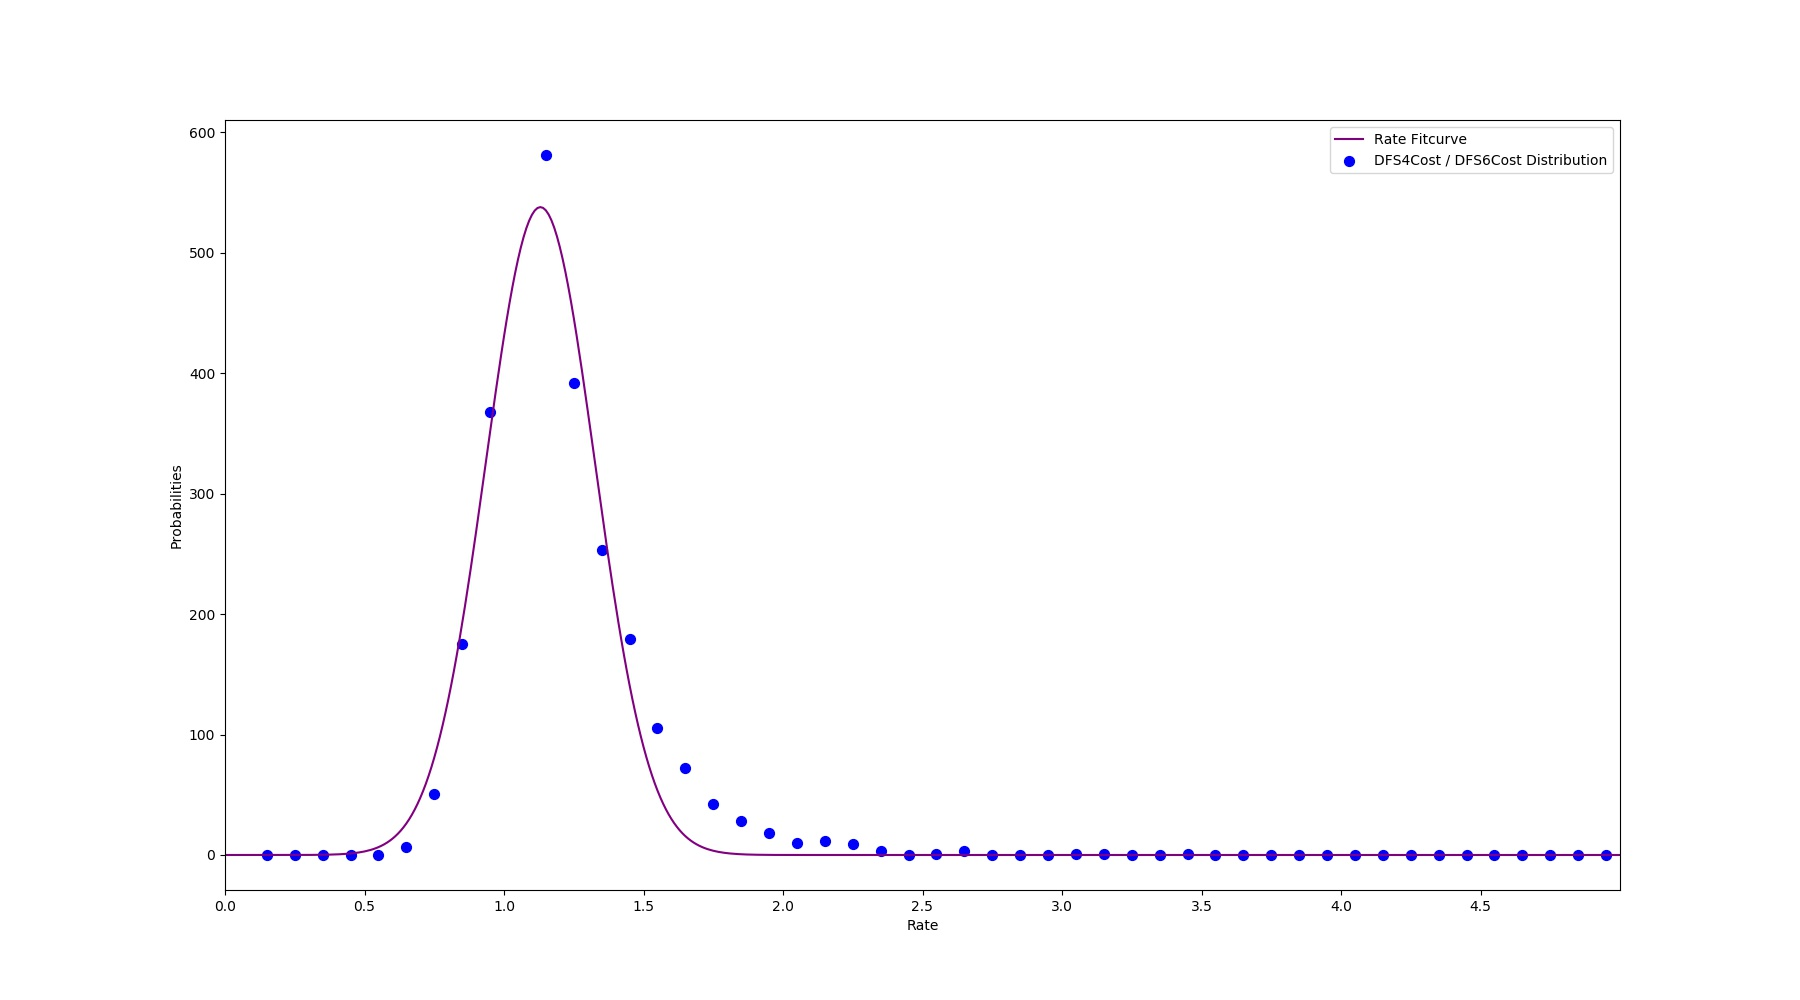
\includegraphics[width=9cm]{graph/cost_dfs4dfs6_norm.jpg}
\caption{Cost Ratio Distribution}
\label{Graph3-1}
\end{minipage}
\begin{minipage}[t]{0.48\textwidth}
\centering
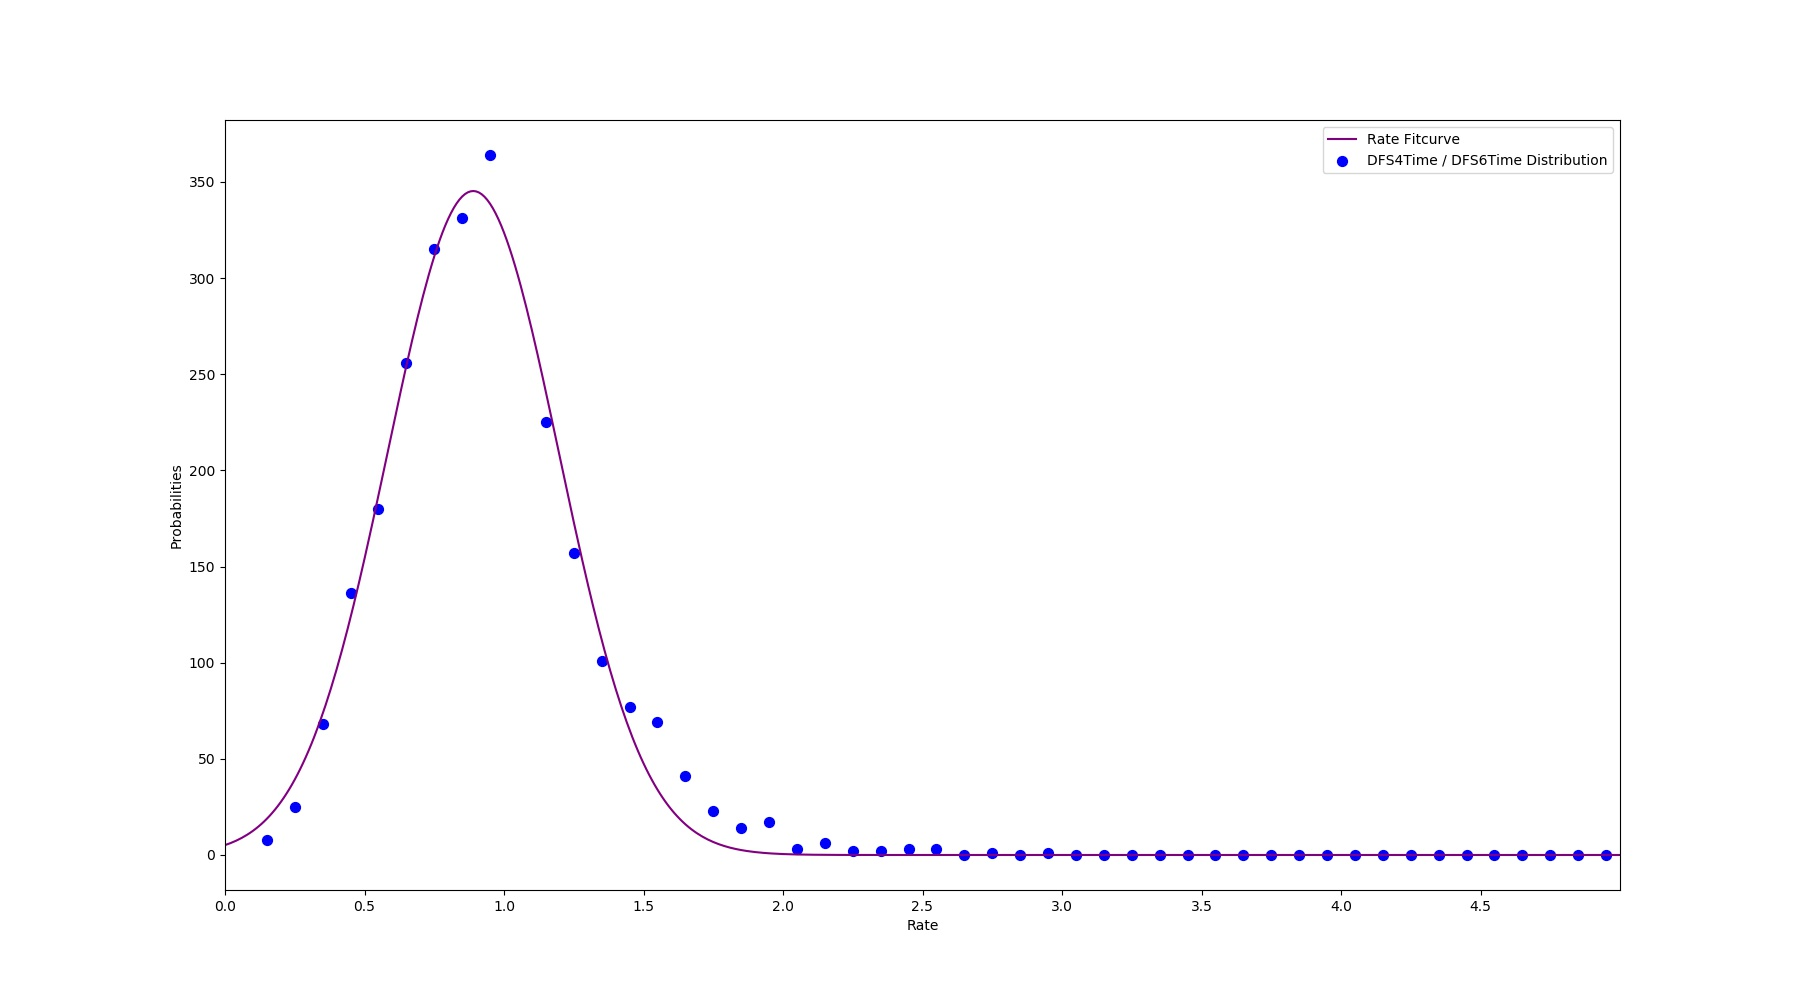
\includegraphics[width=9cm]{graph/time_dfs4dfs6_norm.jpg}
\caption{Time Ratio Distribution}
\label{Graph3-2}
\end{minipage}
\end{figure}

With regard to program running efficiency, we give the unit cost distribution(Figure.~\ref{Graph3-0-0}) to express. In this graph, we can find that with DFS depth increase, the concentration of fixed normalization is becoming centered as well. According to Three-Sigma Rule of Thumb, orders will transfer with lower cost if we use larger depth(variance becoming lower).

As is mentioned above, as we use IDDFS with depth=4, we can get 2-approximation optimal solution with relatively high efficiency.

\par 

\newpage
\section{Problem 2}
\subsection{Problem Analysis}
In this section, we set some hubs in some cities. Hubs can gather packages and send them together to the same city with lower unit cost. However, the packages gathered together at a hub to one
destination can only be sent by one transportation tool. We defined some new symbols \\
\begin{table}
  \caption{Problem 2 Symbols}\label{sym2}
  \centering
  \begin{tabular}{|l|l|}
  \hline
  Symbol &  Definition \\
  \hline
  $\hat{C}$ & The cost of setting a hub, a constant\\
  \hline
  $discount$ & The discount rate on the cost when packages are sent from the same hub, $discount\in (0,1)$\\
  \hline
  $\#hub$ & The number of hubs \\
  \hline
  $H$ & The set of cities where hubs are set \\
  \hline
  \end{tabular}
\end{table}
We consider it's an $NPO$ problem as well.
\begin{itemize}
  \item $I$: The network model $G=(V,E)$, the set of $order$, the set of hubs $H$
  \item $sol$: A set of paths $P$ representing the delivery scheme
  \item $m$: $m(G,order,H,\hat{C},discount)=\sum_{p \in P}C(p)+\#hubs\times\hat{C}$.
  \item $goal$: $min$
\end{itemize}
\subsection{Algorithm Design}
First, we designed the algorithm to choose suitable cities to set hubs. Our strategy to select hubs is to sort the degree, including the in-degree and out-degree, and find the largest $\#hubs$ and add to the set of hubs $H$. The intuition of selecting this strategy is that 
Then, we designed the algorithm to find a new delivery scheme.
\begin{algorithm}
  \KwIn{$G$, $out\_ways\_of\_hub$, $source\_city$, $target\_city$, $order\_time$, $arrival\_time$
        , $visited[]$, $path$, $min$, $optimal\_path$, $depth\_limit$}
  \BlankLine
  \caption{dfs with hubs}
  \label{Alg-dfs-with-hubs}
  
  \If{$source\_city == target\_city$ and $path$'s value $< min$ }{
    $min=$ $path$'s value\;
    $optimal\_path = path$\;
    $return$\; 
  }
  \If{$depth\_limit ==0$}{
    $return$\;
  }
  \BlankLine 
  
  $visited[source\_city] = true$\;
  \If{$source\_city$ is hub}{
    \For{each $(city, out\_way)$ adjacent
         to $source\_city$ in Graph $out\_ways\_of\_hub$}{
      \If{$visited[city]==true$ 
          and $out\_way.departure\_time \ge arrival\_time$}{
            $visited[city] = true$\;
            $path.push\_back(out\_way)$\;
            \BlankLine
            \If{$path$'s value $< min$}{
              $dfs(G,out\_ways\_of\_hub , city, target\_city, order\_time, out\_way.arrival\_time$\\
              $, visited, path, min, optimal\_path, depth\_limit - 1)$\;
            }
            \BlankLine
            $path.pop\_back()$\;
            $visited[city] = false$\;
          }
    }
  }
  \Else{
    \For{each $(city, out\_way)$ adjacent to $source\_city$ in Graph G}{
      \If{$visited[city]==true$ 
          and $out\_way.departure\_time \ge arrival\_time$}{
            $visited[city] = true$\;
            $path.push\_back(out\_way)$\;
            \BlankLine
            \If{$path$'s value $< min$}{
              $dfs(G, city, target\_city, order\_time, out\_way.arrival\_time$\\
              $, visited, path, min, optimal\_path, depth\_limit - 1)$\;
            }
            \BlankLine
            $path.pop\_back()$\;
            $visited[city] = false$\;
          }
    }
  }

\end{algorithm}
\subsection{Theoretical Analysis}
\subsubsection{Complexity Analysis}
The time complexity is the same as the Problem 1. So we simply omit the analysis here and just give the result. We use the same notation as before, the time complexity is $O((\dfrac{b}{2})^d)$.
\subsubsection{Efficiency Analysis}
Also it's an NP problem which is easy to verify (can find a poly-time certifier)
\subsection{Performance Evaluation}

\begin{figure}[htbp]
  \centering
  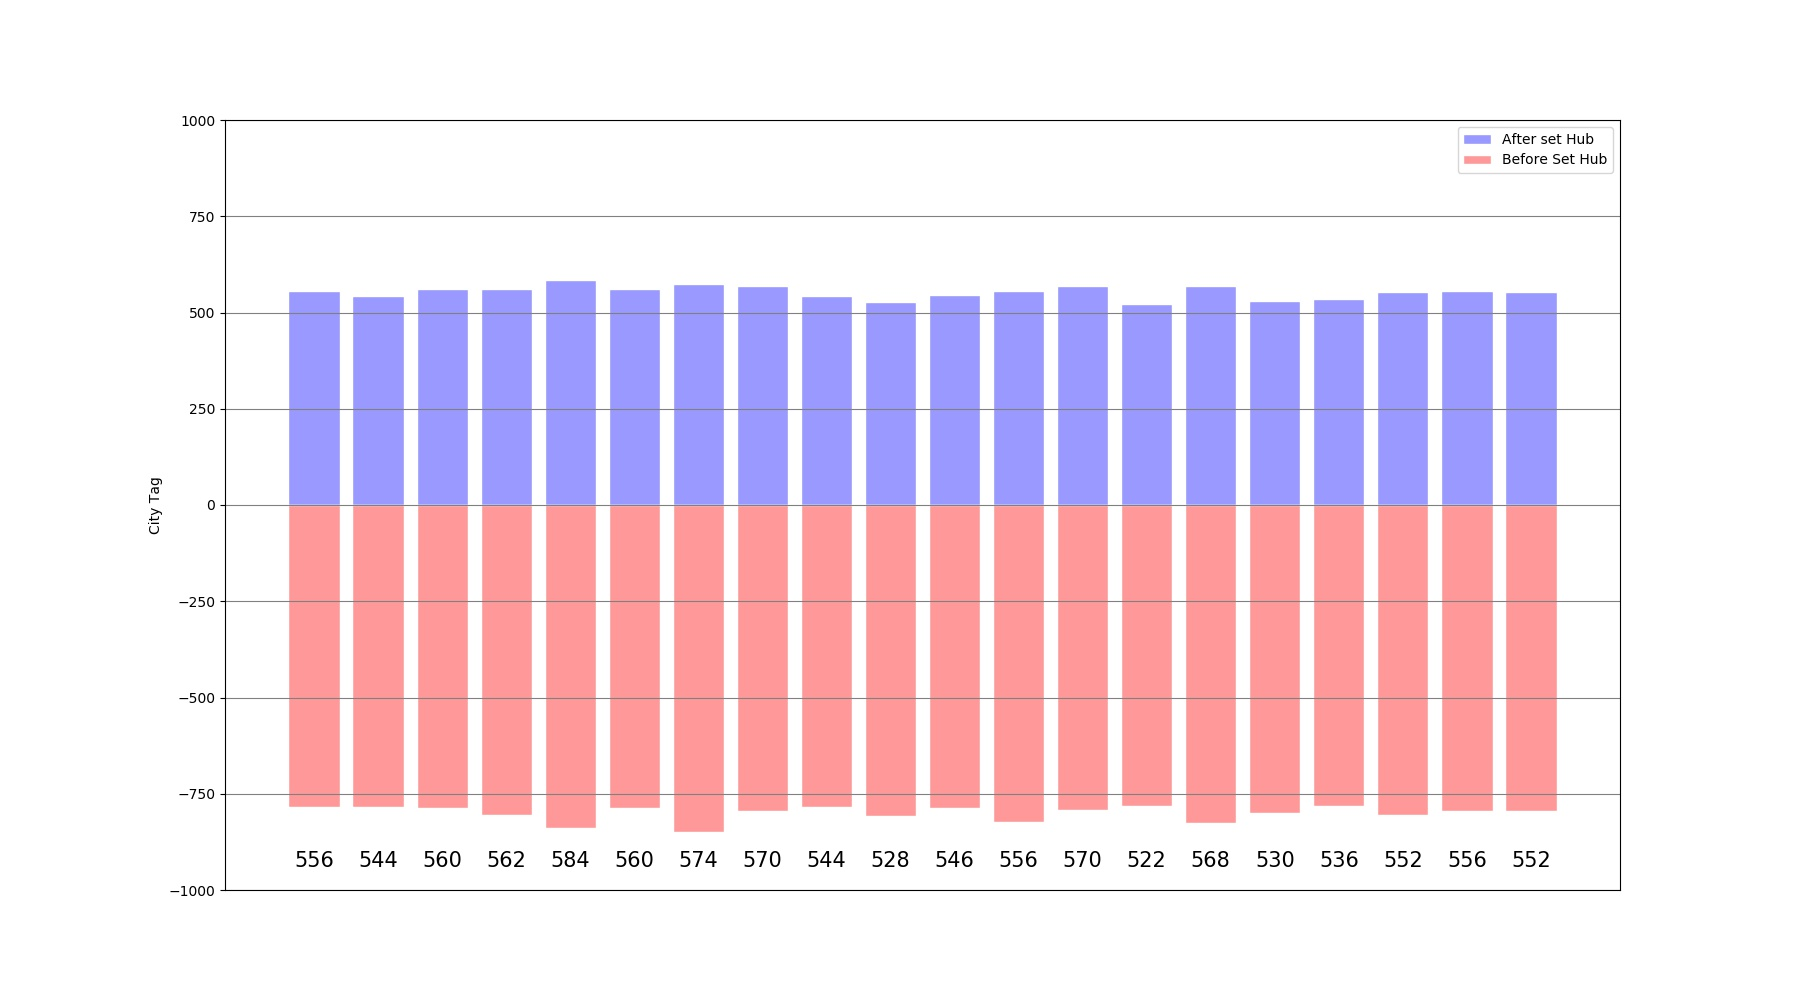
\includegraphics[height = 5cm]{graph/DegreeChange.jpg}
  \caption{Hub Degree}
  \label{bargraph0}
\end{figure}

As we select hub by sorted degree and under the constrain that all the orders sent from a hub can use only one transportation method. We can select the selected hubs and see its degree changes in Figure.~\ref{bargraph0}. All the degree of every hub decreased because constrains is added.\par

In Figure.~\ref{Graph4-1} and Figure.~\ref{Graph4-2}, We respectively use polynomial function and normalization function to fix the Time Ratio Distribution over no-hub case and 20-hub case, according to the integral function of the fixed curve, we can claim that if we add the first 20 most degree hub, more than $60\%$ percent of orders cost more time than previous because we make a discount on out-sent fare of every hub, which makes weight get to cost rather than time according to Figure.~\ref{fig:rt}.\par

\begin{figure}[htbp]
\centering
\begin{minipage}[t]{0.48\textwidth}
\centering
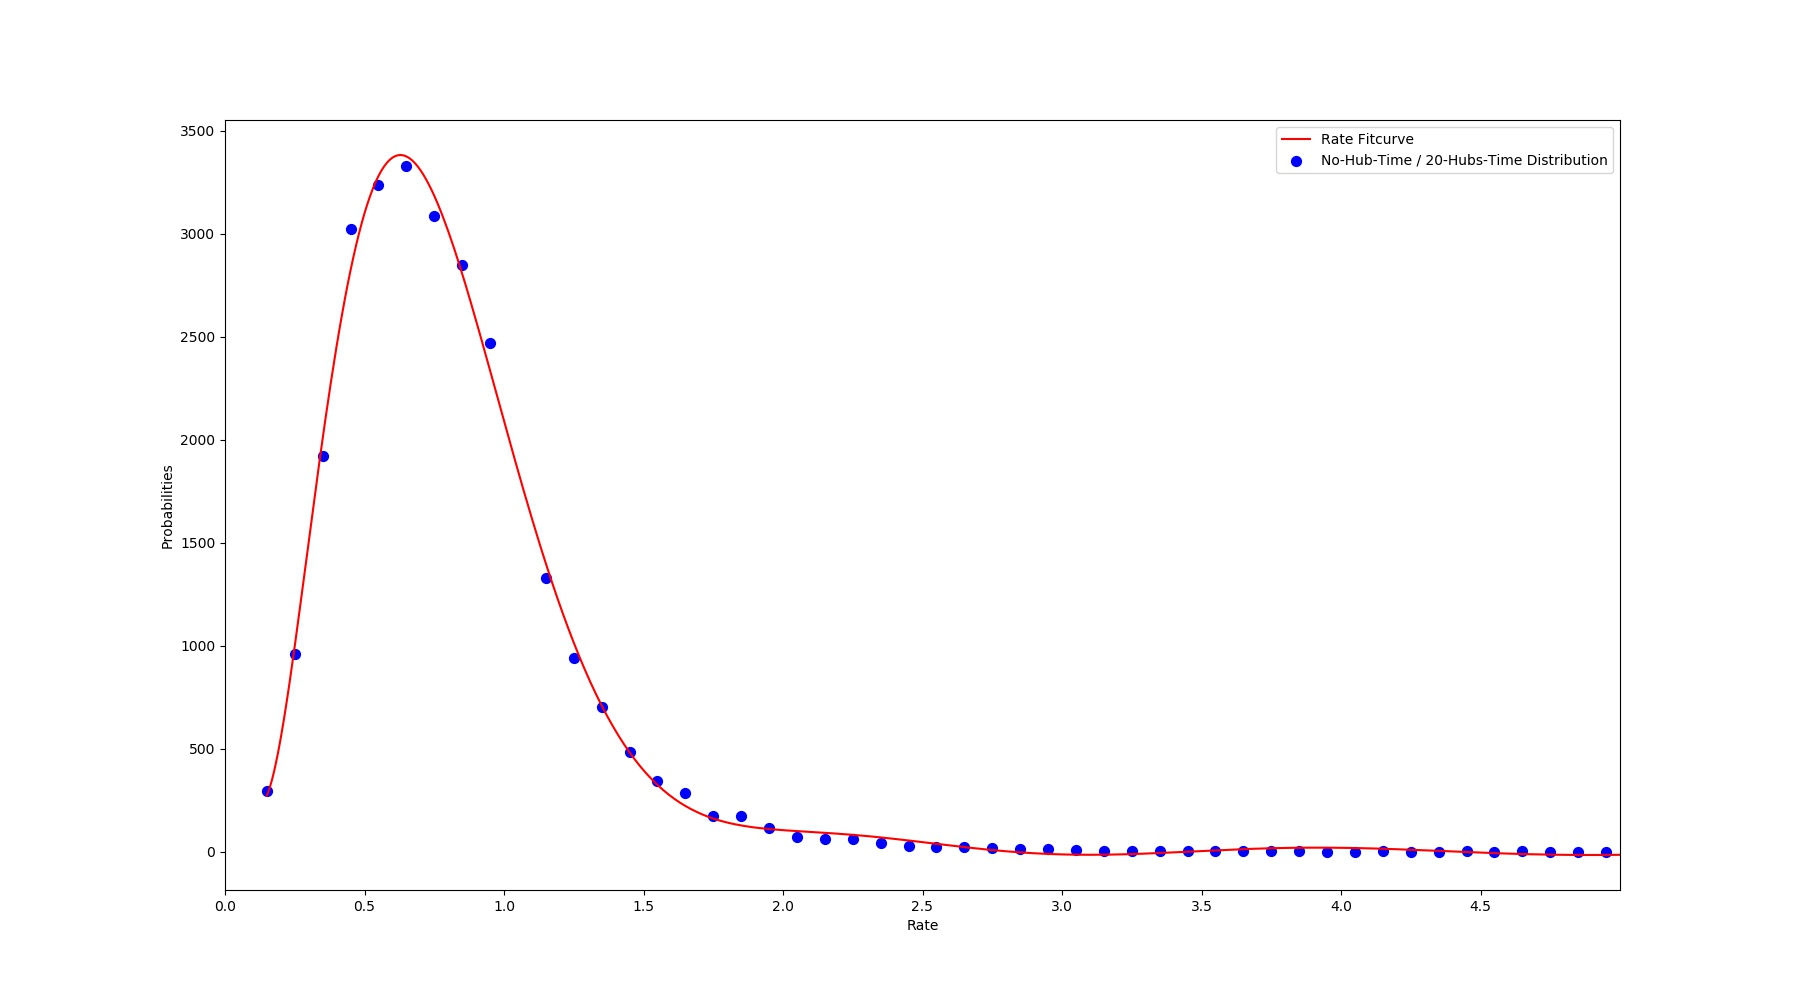
\includegraphics[width=9cm]{graph/time_pro1pro2_poly.jpg}
\caption{Time Ratio With Poly Fix}
\label{Graph4-1}
\end{minipage}
\begin{minipage}[t]{0.48\textwidth}
\centering
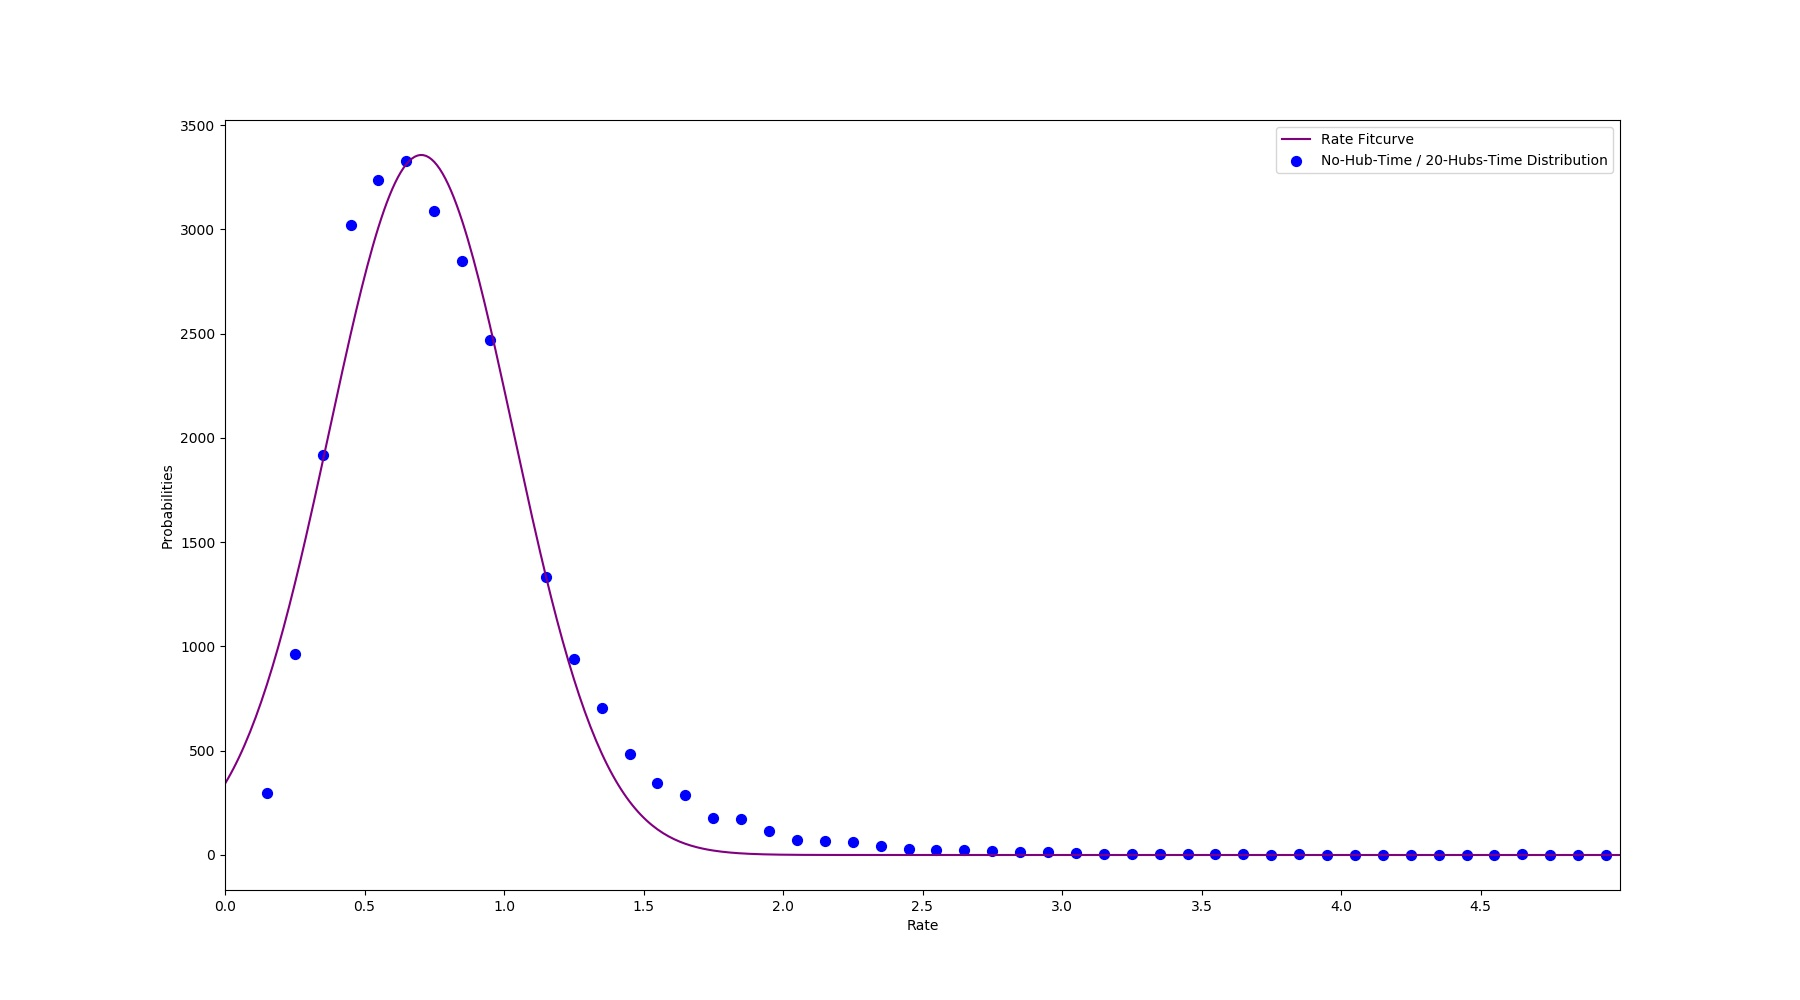
\includegraphics[width=9cm]{graph/time_pro1pro2_norm.jpg}
\caption{Time Ratio with Normalization Fix}
\label{Graph4-2}
\end{minipage}
\end{figure}

Correspondingly, Cost Ratio function will shift right to have more cost increase as Figure.~\ref{Graph4-1} and Figure.~\ref{Graph4-2}. Obviously, Normalization fix curve have a better performances.

\begin{figure}[htbp]
\centering
\begin{minipage}[t]{0.48\textwidth}
\centering
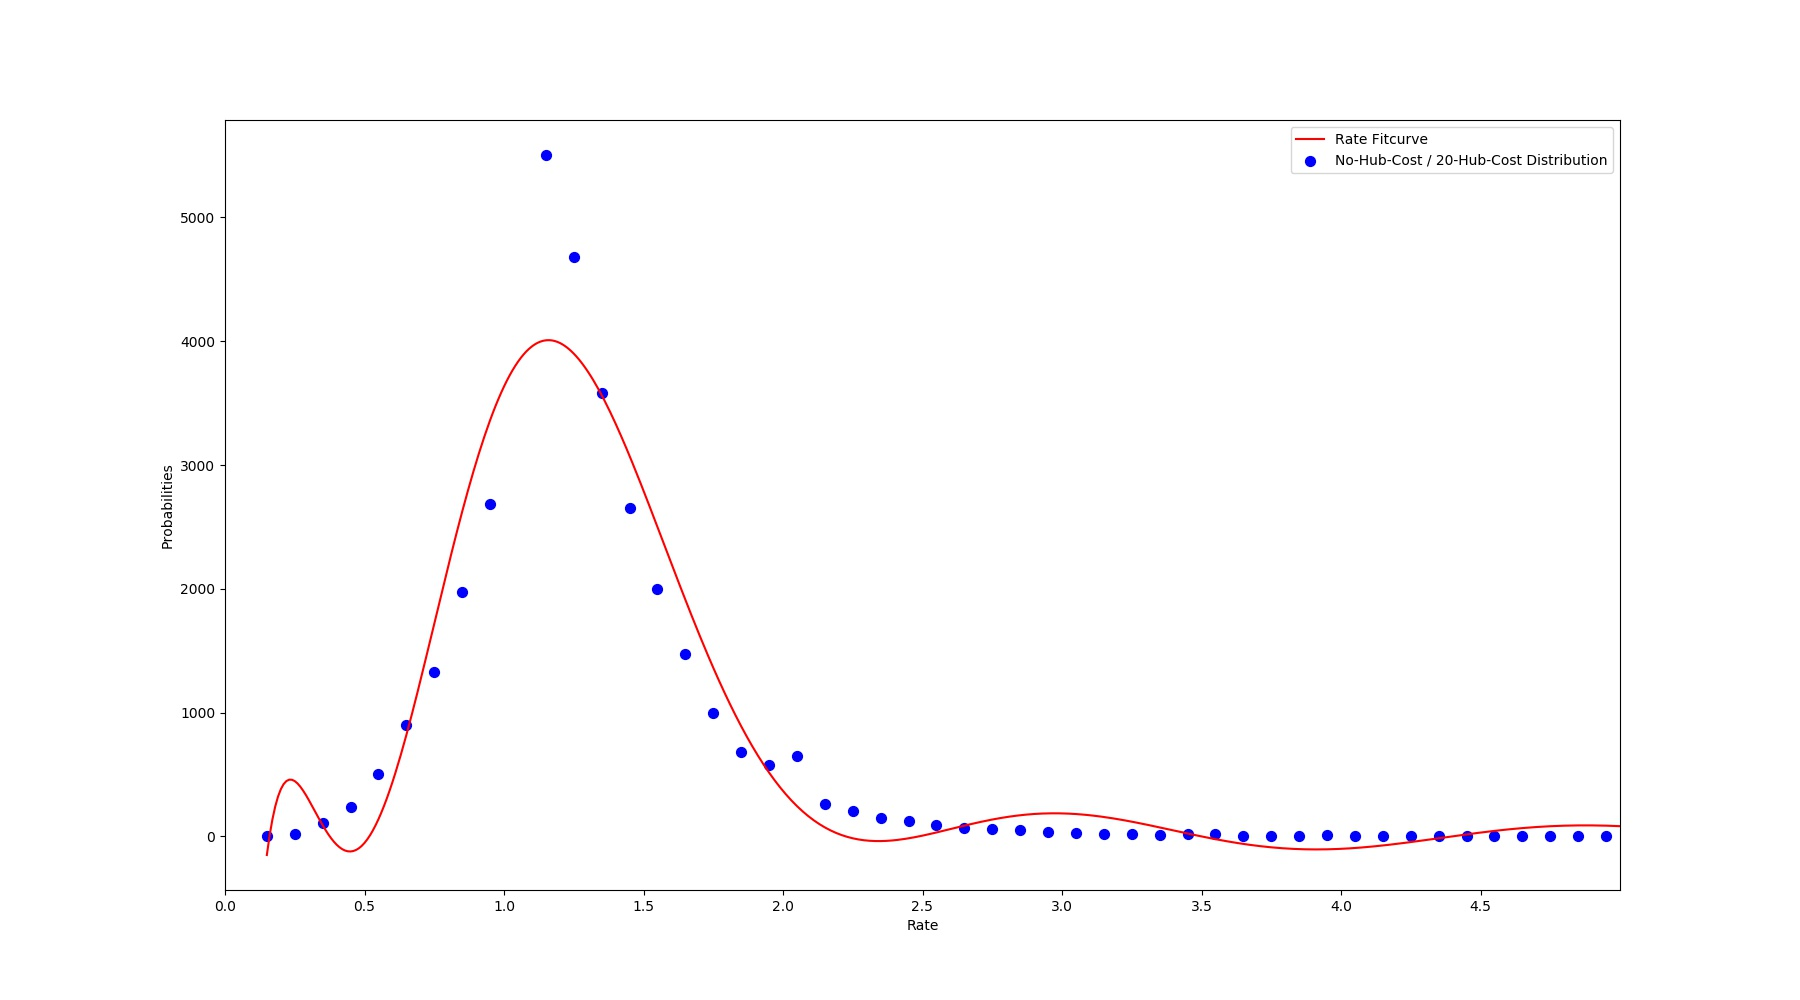
\includegraphics[width=9cm]{graph/cost_pro1pro2_poly.jpg}
\caption{Cost Ratio With Poly Fix}
\label{Graph5-1}
\end{minipage}
\begin{minipage}[t]{0.48\textwidth}
\centering
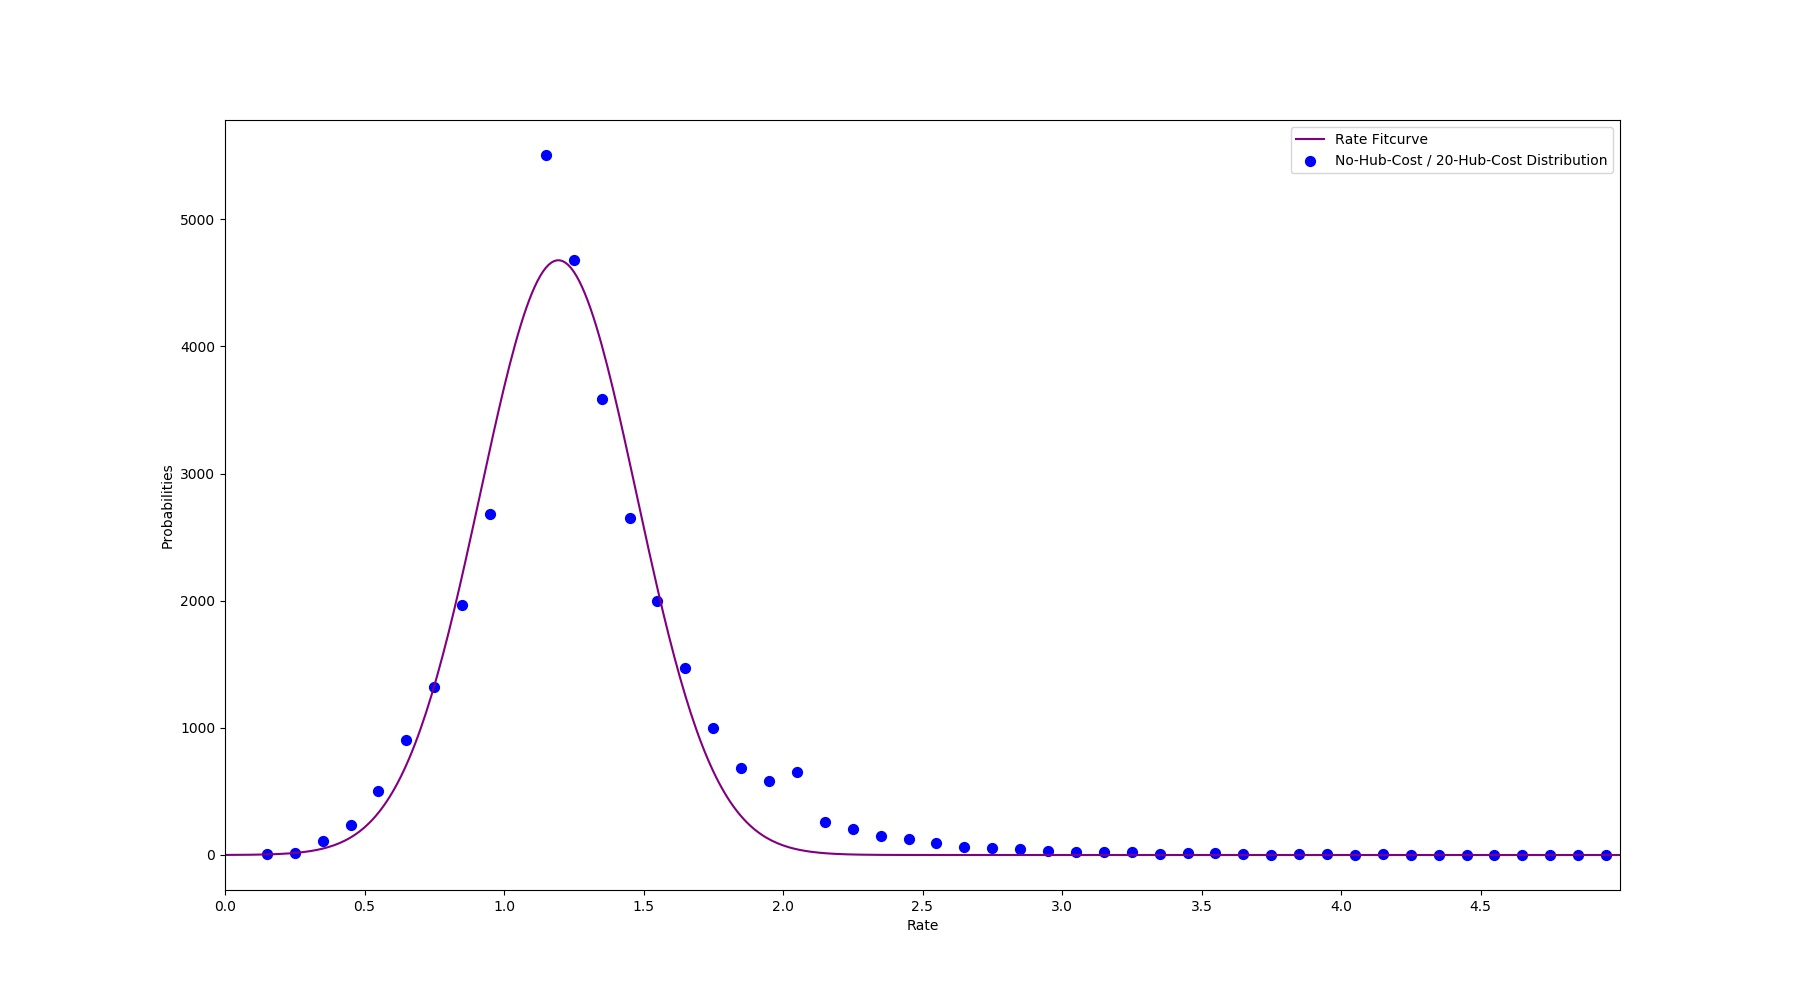
\includegraphics[width=9cm]{graph/cost_pro1pro2_norm.jpg}
\caption{Cost Ratio with Normalization Fix}
\label{Graph5-2}
\end{minipage}
\end{figure}

In this part, we use a hub selection algorithm and hub discount filter, we can get the total transportation cost 134529178.7 CNY with relatively high efficiency.

\newpage
\section{Problem 3}
\subsection{Problem Analysis}
In real case, some other constraints should be considered: the hubs may be capacitated; some hubs may not accept some specific packages; some packages
may not be transferred by some transportation tools. We listed our constraints for transportations as follows \par
\begin{table}
  \caption{Constraints on Transportations}\label{cts1}
  \centering
  \begin{tabular}{|l|l|}
  \hline
  Tool &  Constraint \\
  \hline
  Trunk & None\\
  \hline
  Train & None\\
  \hline
  Plane & Inflammable Products, Liquid \\
  \hline
  Ship & Food \\
  \hline
  \end{tabular}
\end{table}
As for constraints on hubs, we randomly set some constraints on hubs. Here, the problem is still an $NPO$, we just add some new constraints to it.
And we still cannot convert it to $LP$ or $ILP$.
\subsection{Algorithm Design}
\begin{algorithm}
  \KwIn{$G$, $source\_city$, $target\_city$, $order\_time$, $arrival\_time$
        , $visited[]$, $path$, $min$, $optimal\_path$, $depth\_limit, commodity\_type$}
  \BlankLine
  \caption{dfs with constraints}
  \label{Alg-dfs-with-constraints}
  
  \If{$source\_city == target\_city$ and $path$'s value $< min$ }{
    $min=$ $path$'s value\;
    $optimal\_path = path$\;
    $return$\; 
  }
  \If{$depth\_limit ==0$}{
    $return$\;
  }
  \BlankLine 
  
  $visited[source\_city] = true$\;
  \For{each $(city, out\_way)$ adjacent to $source\_city$}{
    \If{$visited[city]==true$ 
        and $out\_way.departure\_time \ge arrival\_time$
        and $out\_way.type$ can deliver $commodity\_type$}{
          $visited[city] = true$\;
          $path.push\_back(out\_way)$\;
          \BlankLine
          \If{$path$'s value $< min$}{
            $dfs(G, city, target\_city, order\_time, out\_way.arrival\_time$\\
            $, visited, path, min, optimal\_path, depth\_limit - 1, commodity\_type)$\;
          }
          \BlankLine
          $path.pop\_back()$\;
          $visited[city] = false$\;
        }
  }

\end{algorithm}
\subsection{Theoretical Analysis}
However, we failed to implement our algorithm when we add capacities to the hubs. We are implementing a sequential algorithm, which means once an order is considered and the optimal or suboptimal solution is found, we will never change it later on. Thus, we cannot compute the certain number of packages residing in a certain hub for a certain time slot and then change the delivery scheme. But we found another way to estimate the extra cost when the capacity is added. We can count the number of packages a hub dealt with in a certain time slot and scale it with a weight then add it to the cost of setting a hub. Then, although we cannot simulate the delivery on our network, we can roughly estimate the effect of hub capacity.
%\newpage
\section{Problem 4}
\subsection{Problem Analysis}
In this problem, we suppose that the SF Express does not have substations in all cities, but only in big cities. Here we suppose that the big cities are those supporting airline service. 
This means that the SF Express should first take the packages from sellers to some substations, and when delivering the packages to purchasers, some substations should receive the packages first, and then send them to the city that the purchasers are in.
\subsection{Algorithm Design}
In our algorithm, we first take packages to the big cities. Then we have two choices, one for leaving this city for the destination, another for carrying on walking among those big cities. This implies the state transition diagram Figure.\ref{fig:fm} in IDDFS recursion.
\begin{algorithm}
  \KwIn{$G\_among\_big\_cities$, $G\_other\_routes$, $source\_city$, $target\_city$, $order\_time$, $arrival\_time$
        , $visited[]$, $path$, $min$, $optimal\_path$, 
        $depth\_limit\_search\_for\_big$, $depth\_limit\_among\_big$, $depth\_limit\_leave\_from\_big$}
  \BlankLine
  \caption{dfs for deliveries only happen between big cities}
  \label{Alg-dfs-for-deliveries-only-happen-between-big-cities1}
  
  \If{$source\_city == target\_city$ and $path$'s value $< min$ }{
    $min=$ $path$'s value\;
    $optimal\_path = path$\;
    $return$\; 
  }
  \BlankLine 
  
  //has not been in big cities (in the stage of searching for big cities)\;
  \If{source\_city is not big cities}{
    //search for a big city\;
    \If{depth\_limit\_search\_for\_big $ne 0$}{
      $visited[source\_city] = true$\;
      \For{each $(city, out\_way)$ adjacent to $source\_city$ 
      in Graph $G\_other\_routes$}{
        \If{$visited[city]==true$ 
            and $out\_way.departure\_time \ge arrival\_time$}{
              $visited[city] = true$\;
              $path.push\_back(out\_way)$\;
              \BlankLine
              \If{$path$'s value $< min$}{
                dfs($G\_among\_big\_cities$, $G\_other\_routes$, $source\_city$, $target\_city$, $order\_time$, $arrival\_time$
        , $visited[]$, $path$, $min$, $optimal\_path$, 
        $depth\_limit\_search\_for\_big - 1$, $depth\_limit\_among\_big$, $depth\_limit\_leave\_from\_big$)\;
              }
              \BlankLine
              $path.pop\_back()$\;
              $visited[city] = false$\;
            }
      }
    }
  }
\end{algorithm}
%\newpage
\begin{algorithm}
  \BlankLine
  \caption{dfs for deliveries only happen between big cities}
  \label{Alg-dfs-for-deliveries-only-happen-between-big-cities}
  // has been in big cities\;
  \Else{
    \BlankLine
    // we can go to another big city\;
    \If{depth\_limit\_among\_big $ne 0$}{
      $visited[source\_city] = true$\;
      \For{each $(city, out\_way)$ adjacent to $source\_city$ 
      in Graph $G\_among\_big\_cities$}{
        \If{$visited[city]==true$ 
            and $out\_way.departure\_time \ge arrival\_time$}{
              $visited[city] = true$\;
              $path.push\_back(out\_way)$\;
              \BlankLine
              \If{$path$'s value $< min$}{
                dfs($G\_among\_big\_cities$, $G\_other\_routes$, $source\_city$, $target\_city$, $order\_time$, $arrival\_time$
        , $visited[]$, $path$, $min$, $optimal\_path$, 
        $0$, $depth\_limit\_among\_big - 1$, $depth\_limit\_leave\_from\_big$)\;
              }
              \BlankLine
              $path.pop\_back()$\;
              $visited[city] = false$\;
            }
      }
    }

    \BlankLine
    // Also, we can leave from this big city to the destination\;
    \If{depth\_limit\_leave\_from\_big $ne 0$}{
      $visited[source\_city] = true$\;
      \For{each $(city, out\_way)$ adjacent to $source\_city$ 
      in Graph $G\_other\_routes$}{
        \If{$visited[city]==true$ 
            and $out\_way.departure\_time \ge arrival\_time$}{
              $visited[city] = true$\;
              $path.push\_back(out\_way)$\;
              \BlankLine
              \If{$path$'s value $< min$}{
                dfs($G\_among\_big\_cities$, $G\_other\_routes$, $source\_city$, $target\_city$, $order\_time$, $arrival\_time$
        , $visited[]$, $path$, $min$, $optimal\_path$, 
        $0$, $0$, $depth\_limit\_leave\_from\_big - 1$)\;
              }
              \BlankLine
              $path.pop\_back()$\;
              $visited[city] = false$\;
            }
      }
    }
  }
        

\end{algorithm}
\newpage
The state transition diagram of the algorithm is shown as follows:
\begin{figure}[htbp]
  \centering
  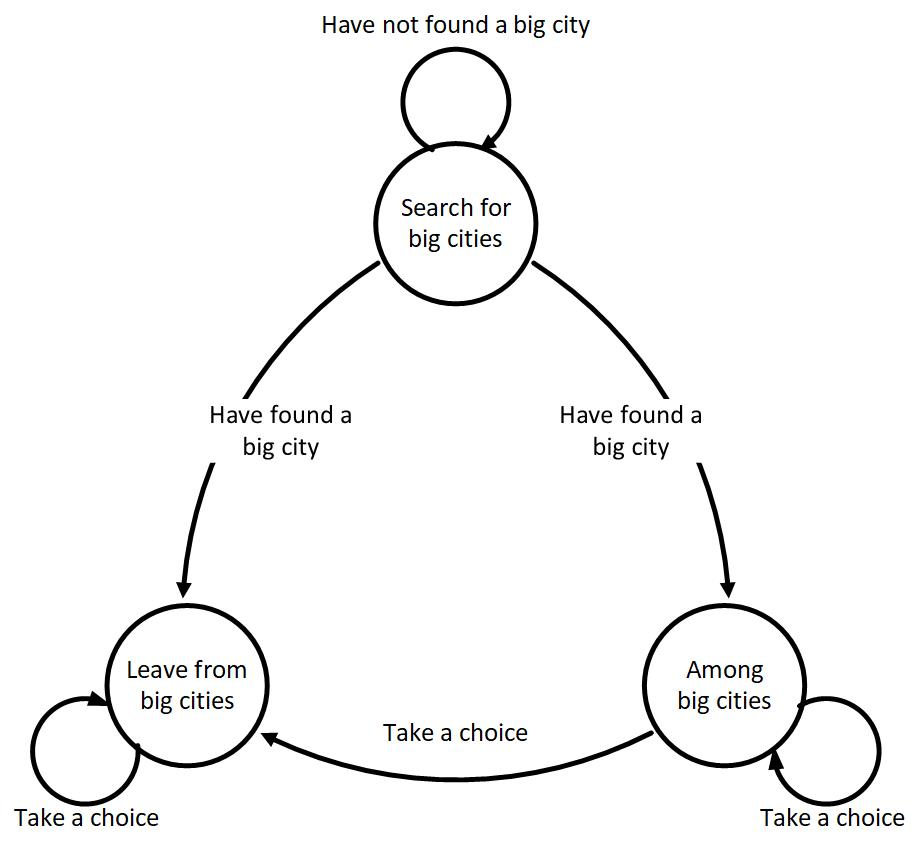
\includegraphics[height = 8cm]{graph/FM.jpg}
  \caption{State Transition Diagram}
  \label{fig:fm}
\end{figure}
\subsection{Theoretical Analysis}
We designed a new algorithm in this part. However, the graph does not change, the sketch of our algorithm is still IDDFS and the depth does not change. The new requirements can be regarded as some kind of constraints added to our model. We can just follow the analysis in Problem 1 and thus the time complexity is $O((\dfrac{b}{2})^d)$ using the same notation as before.
\subsection{Performance Evaluation}
In this part, I will give an analysis about the algorithm we design, we write an simulator in C++ to process every order and give the OPT ratio distribution in Figure.~\ref{Graph6-1} and Figure.~\ref{Graph6-2}.

\begin{figure}[htbp]
\centering
\begin{minipage}[t]{0.48\textwidth}
\centering
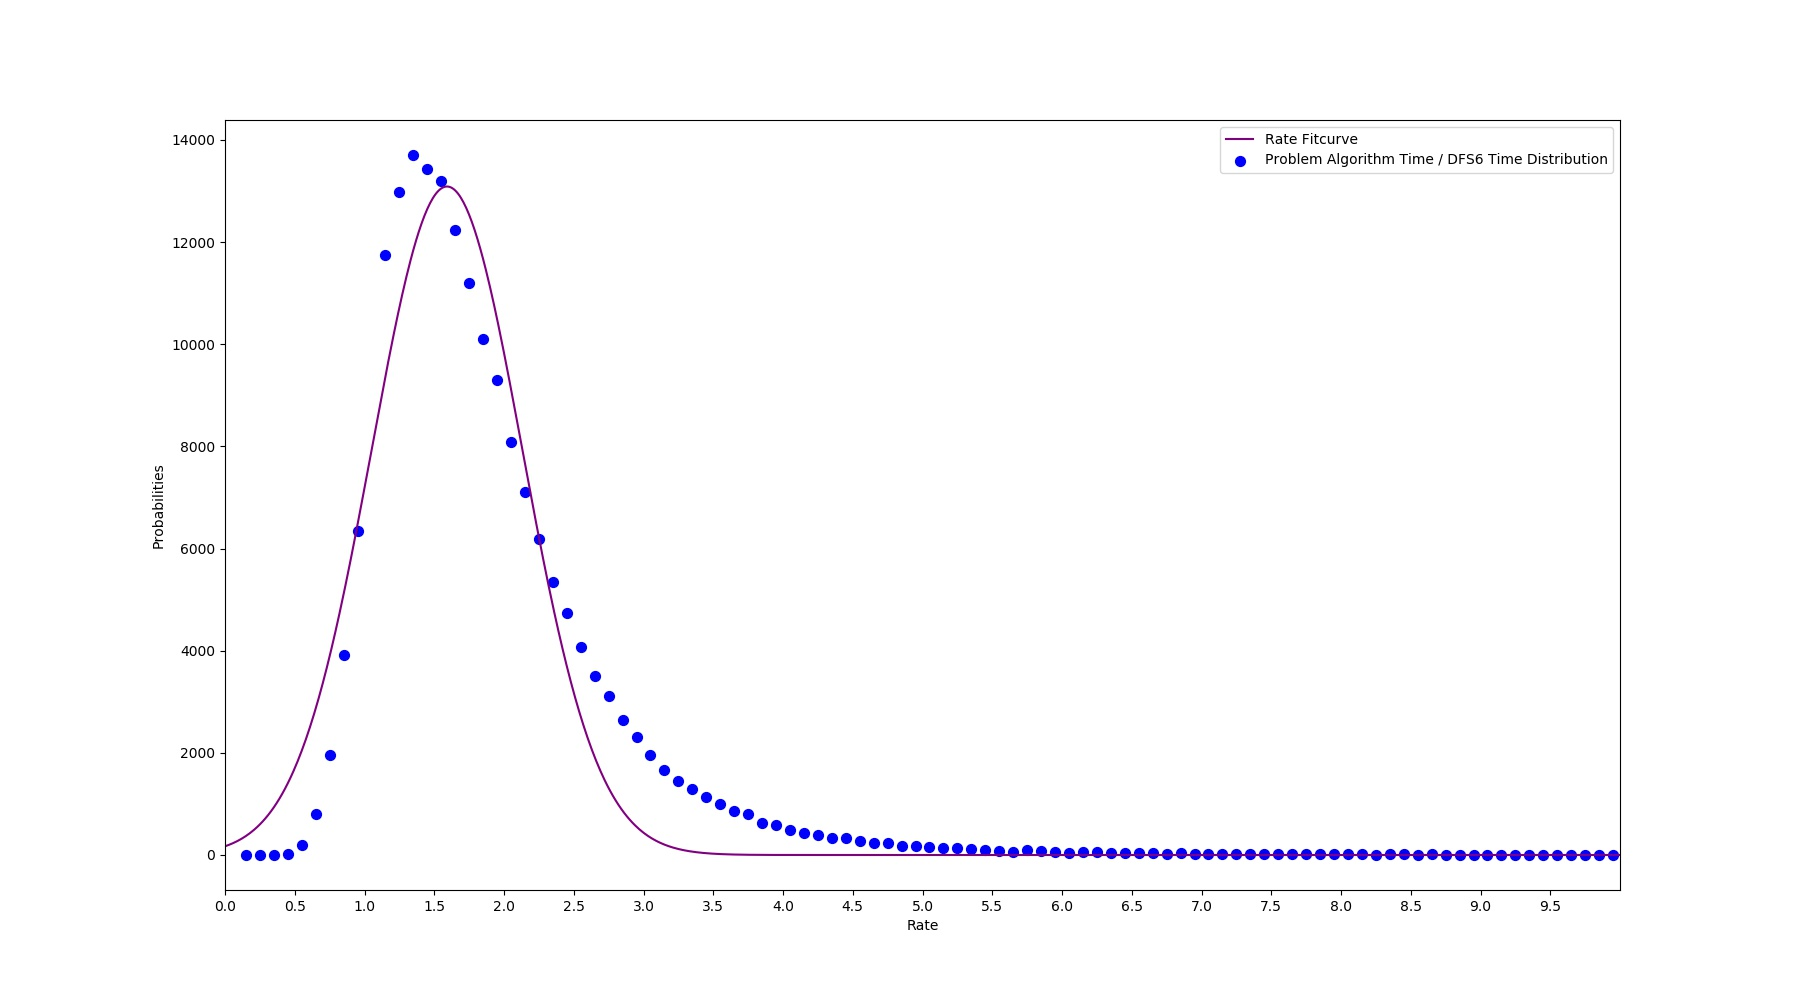
\includegraphics[width=9cm]{graph/cost_prob4.jpg}
\caption{Cost OPT Ratio Distribution}
\label{Graph6-1}
\end{minipage}
\begin{minipage}[t]{0.48\textwidth}
\centering
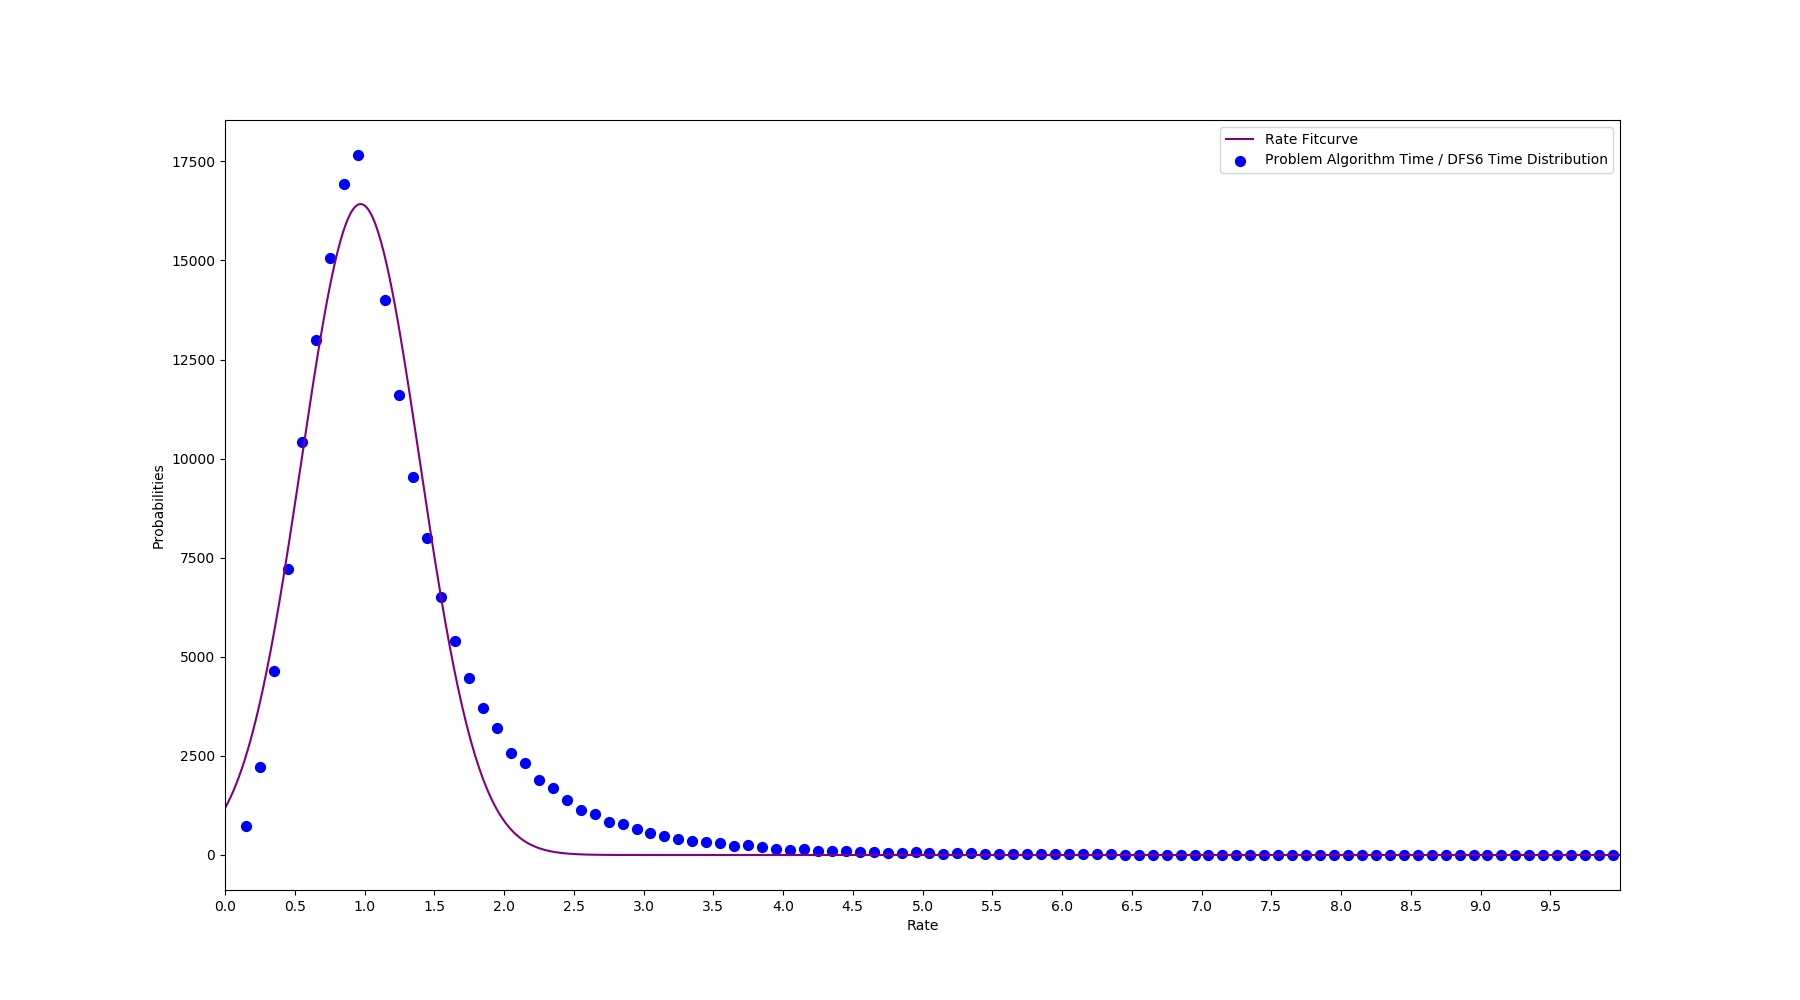
\includegraphics[width=9cm]{graph/time_prob4.jpg}
\caption{Time OPT Ratio Distribution}
\label{Graph6-2}
\end{minipage}
\end{figure}

We can see that Time Distribution and Cost Distribution is strictly bounded by 4, while the Time Distribution's mean expectation equals 1. It means the time we cost neither increase nor decrease overall(according to Law of Large Number), while Cost is bounded by a constant value($80\%$ bounded by 2, $100\%$ bounded by 4). And our final result is 217822952.19(DFS6 in Problem 1 is 134529178.70, approximate ratio works).

\section*{Acknowledgements}
In this project, we designed the model and algorithms to solve the package delivery problem and then analysed the performance of our algorithm. We made use of graph algorithms, approximation algorithms and their analysis that we learned from the lecture. We met a lot of difficulties during these days. At first, we tried to formulate the problem into LP or ILP, but we found it's really hard to cope with the time including the order time, the departure time and so on. Then, we decide to construct a network model and apply graph algorithms on it. After that, we designed a modified DFS algorithm to search for the feasible solution. Then, we found that it's really computational expensive, because the input size is huge. We upload our program to our server and run them day and night. We spent most of time solving and analysing the first problem and when it comes to Problem 3, we found that our algorithm cannot work to find the solution when capacity of hubs are set. Above all, we practiced our skills of designing models and algorithms and analyzing algorithms. We understand that an efficient algorithm is significant when facing huge input size. Thanks Prof. Gao for teaching us so many useful algorithms and analyzing skills. We think we will benefit a lot from them in our future study.

%
% ---- Bibliography ----
%
% BibTeX users should specify bibliography style 'splncs04'.
% References will then be sorted and formatted in the correct style.
%
% \bibliographystyle{splncs04}
% \bibliography{mybibliography}
%
\newpage

\begin{thebibliography}{8}
\bibitem{ref_article1}
Correia, I., Nickel, S., \& Saldanha-da-Gama, F. “A stochastic multi-period capacitated multiple allocation hub location problem: Formulation and inequalities.” Omega, 74, 122-134,2018.

\bibitem{ref_lncs1}
Zäpfel, G., \& Wasner, M. "Planning and optimization of hub-and-spoke transportation networks of cooperative third-party logistics providers." International journal of production economics, 78(2), 207-220, 2002.

\bibitem{ref_book1}
Gelareh S, Monemi RN, Nickel S. "Multi-period hub location problems in trans- portation. Transportation Research Part E: Logistics and Transportation" Review 75:67–94, 2015.

\bibitem{ref_proc1}
Alumur, S. A., Nickel, S., Saldanha-da-Gama, F., \& Seçerdin, Y. "Multi-period hub network design problems with modular capacities." Annals of Operations Research, 246(1-2), 289-312, 2016.
\end{thebibliography}
\section*{Appendix}
The source code is at \url{https://github.com/DeanAlkene/CS214-Project}
\end{document}
